\documentclass[11pt]{article} %Tamaño de la letra

%Paquetes esenciales
\usepackage[spanish]{babel}
\usepackage[utf8]{inputenc}
\usepackage[T1]{fontenc}
\usepackage{float}
%Fuente arial
\usepackage{helvet}
\renewcommand{\familydefault}{\sfdefault}

%Hipervinculos y citas
\usepackage{csquotes} %
\usepackage[backend=biber, style=apa, sortlocale=es]{biblatex} % <-- CORREGIDO
\usepackage{hyperref} % <-- CORREGIDO: estaba mal escrito como 'hyperrref'
\usepackage{url}
%Graficos y color
\usepackage{graphicx} % Required for inserting images
\usepackage{xcolor}
\usepackage{tikz}
\usetikzlibrary{arrows.meta}
\usetikzlibrary{positioning}    
\usetikzlibrary{babel}
\usepackage{amsmath}
\usepackage{colortbl}
%Simbologia Matematica
\usepackage{amsmath}
\usepackage{amsfonts} % ← Necesario para \mathbb
\usepackage{amssymb}


%Margenes y espacio
\usepackage[a4paper, left = 2cm, right = 1cm, top=2cm,bottom=2cm]{geometry}
\usepackage{setspace}
\linespread{1.0} %Espacio
\usepackage{setspace}


%Esto cambia el color del fondo
\pagecolor{gray!20} %Cambia este color de las paginas
\color{black} %Cambia el color del texto


%Bibilografia
\addbibresource{referencias.bib}
\begin{document}


% PORTADA
\begin{titlepage}
    \thispagestyle{empty}
    \begin{spacing}{1.5}
    \begin{center}
        
\includegraphics[width=0.2\textwidth]{Images/LogoUNA.svg.png} \\[30pt]
        {\Large \textbf{Universidad Nacional de Costa Rica}} \\[20pt] 
        {\Large Escuela de Informática} \\[20pt]
        {\Large \textbf{Redes Neuronales de Grafos (GNNs)}} \\[20pt]
        {\Large Curso: Estructuras Discretas} \\[20pt]
        {\Large \textbf{Estudiantes a cargo de la investigación:}} \\[10pt]
        {\large Sebastián Garro Granados \\ Joel Brenes Vargas \\ Santiago Jesús Hernández Chaves \\ Efraín Ignacio Retana Segura} \\[20pt]
        {\Large \textbf{Profesor a cargo del curso:}} \\[15pt]
        {\large Carlos Loría-Sáenz} \\[120pt]
        {\Large \textbf{Fecha:}} \\[15pt]
        {\large 17 de abril de 2025}
    \end{center}
    \end{spacing}
\end{titlepage}

% RESUMEN
\newpage
{\large \textbf{Resumen}}  
\vspace{5pt}

Este trabajo presenta una investigación introductoria sobre las redes neuronales de grafos (GNNs, por sus siglas en inglés), una poderosa combinación entre teoría de grafos y aprendizaje automático que ha ganado gran relevancia en la última década. En particular, se estudia una arquitectura específica: las Graph Convolutional Networks (GCNs), las cuales permiten extender los mecanismos de redes neuronales convolucionales (CNNs) al dominio no estructurado de los grafos. Este enfoque resulta especialmente útil en aplicaciones donde los datos tienen relaciones o estructuras subyacentes representables mediante nodos y aristas.

El objetivo principal de esta investigación es ofrecer un marco conceptual básico que permita a estudiantes del curso EIF203 Estructuras Discretas comprender los fundamentos de las GNNs y vincularlos con los contenidos vistos en clase, especialmente los relacionados con grafos y su programación en Python. Para lograrlo, el trabajo incluye una revisión teórica sobre el aprendizaje supervisado con redes neuronales, conceptos fundamentales de grafos, y una justificación del uso de GNNs frente a modelos tradicionales.

Como parte del desarrollo, se presentan ejemplos demostrativos en Python donde se implementa un modelo básico de GCN para resolver una tarea de clasificación de nodos. Estos ejemplos utilizan bibliotecas especializadas y están diseñados para reforzar los aspectos técnicos tratados en el documento. Además, se hace uso de herramientas como GitHub para la gestión del código fuente, Overleaf para la documentación técnica, y entornos de desarrollo compatibles con bibliotecas de aprendizaje profundo.

El informe final busca no solo cumplir con los requerimientos del curso, sino también proporcionar al lector una puerta de entrada clara, aplicada y documentada al fascinante mundo de las redes neuronales de grafos.

\vspace{5pt}
\textbf{Palabras clave:} grafos, redes neuronales, GNN, GCN, aprendizaje automático, aprendizaje supervisado, estructuras discretas, Python,nodos, clasificación de nodos.

\newpage
\tableofcontents
\newpage
\listoftables
\listoffigures
\newpage
{\large \textbf{Introducción}}
\vspace{5pt}
parte de garro
\newpage
{\large \textbf{Conceptos de Grafos y sus Aplicaciones}}
\vspace{5pt}
parte de garro
\newpage
{\section{Conceptos Básicos de ML usando Redes Neuronales (NNs)}} \vspace{10pt}

\subsection{a.Nociones de Machine Learning (ML)}
\vspace{5pt}

\subsubsection{i. Definición} 
\vspace{3pt}

El \textit{Machine Learning} (ML) es una rama de la inteligencia artificial (IA) que se enfoca en el desarrollo de algoritmos capaces de aprender a partir de datos. En el pasado, los sistemas requerían que los programadores escribieran explícitamente cada regla, paso a paso. Sin embargo, con el uso de técnicas de aprendizaje automático, las computadoras pueden identificar patrones y relaciones en los datos sin necesidad de intervención directa por parte del programador~\cite{sanchez}. Así, un modelo puede tomar decisiones o hacer predicciones sobre nuevos datos basándose en lo aprendido durante su entrenamiento.

Una de las principales ventajas del \textit{machine learning} es su capacidad para construir modelos matemáticos que representan con precisión las relaciones entre variables, incluso cuando estas no son evidentes o no pueden derivarse de principios lógicos~\cite{amazon2024}.




\vspace{8pt}
\subsubsection{ii. Features y Datasets}\vspace{2pt}
\begin{itemize}
\item \textbf{Features}: Los features (o atributos en español) son las variables que describen cada ejemplo y que el modelo utiliza como entrada para aprender. Pueden proceder directamente de los datos originales (por ejemplo, edad, temperatura) o derivarse mediante \textit{feature engineering}, proceso que consiste en crear una versión más optimizada de estos features transformándolos desde su forma cruda o \textit{raw}~\cite{googleML2025}.
\end{itemize}

\begin{table}[h]
\centering
\caption{Ejemplo simple de \textit{features}. \textit{Fuente: Elaboración propia.}}

\label{tab:simple_features}
\begin{tabular}{|c|c|c|c|}
\hline
\textbf{Edad} & \textbf{Salario} & \textbf{Experiencia} & \textbf{Aprobado} \\
\hline
25 & 30000 & 2 & No \\
\hline
35 & 50000 & 8 & Sí \\
\hline
28 & 35000 & 3 & No \\
\hline
\end{tabular}
\end{table}

\begin{itemize}
    \item \textbf{Dataset}: un \textit{dataset} es la colección organizada de ejemplos sobre los que entrenamos y evaluamos el modelo. Muchos datasets se representan en tablas (por ejemplo, CSV o DataFrames), donde cada fila es un ejemplo y cada columna es un \textit{feature} o una etiqueta(\textit{label}). También pueden provenir de otros formatos como archivos de logs o protocolos binarios. Es importante para el \textit{machine learning} (ML) dividir el \textit{dataset} en subconjuntos de entrenamiento, validación y prueba para garantizar que el modelo generalice correctamente datos nuevos ~\cite{googleML2025}.
\end{itemize}

\begin{table}[h]
\centering
\caption{Ejemplo de dataset en formato CSV para aprendizaje automático. Incluye temperaturas como \textit{features} y el estado de salud como \textit{label}. \textit{Fuente: Elaboración propia, inspirada en el video \textit{Intro Python Parte 03 (2022-02-23)} de Carlos Loría-Sáenz.}}

\label{tab:ml_dataset_example}
\begin{tabular}{|c|c|c|c|c|}
\hline
\textbf{Temp 1} & \textbf{Temp 2} & \textbf{Temp 3} & \textbf{Estado} \\
\hline
37.0 & 37.9 & 37.0 & Sano \\
37.0 & 40.0 & 36.0 & Sano \\
41.0 & 42.0 & 37.0 & Enfermo \\
\hline
\end{tabular}
\end{table}
\vspace{8pt}
\subsubsection{iii. Entrenamiento}
Es el proceso en el cual un modelo ajusta sus parámetros internos -principalmente los pesos de sus conexiones- con el objetivo de minimizar un error o función de pérdida~\cite{nvidia}. Este proceso requiere de una base de datos etiquetada (en el caso de aprendizaje supervisado) y un algoritmo de optimización, siendo el más común \textit{descenso por el gradiente} (\textit{gradient descent})~\cite{sanchez}.

Durante el entrenamiento, el modelo realiza predicciones sobre los datos de entrada y compara sus resultados con las salidas reales. Con base en esa comparación, se calcula el error y se utiliza una técnica llamada \textbf{retropropagación del error} (\textit{backpropagation}) para distribuir este error hacia atrás a través de las capas de la red. Este mecanismo permite que cada peso se ajuste de forma proporcional al impacto que tuvo en el error final.
\begin{figure}[H]
    \centering
    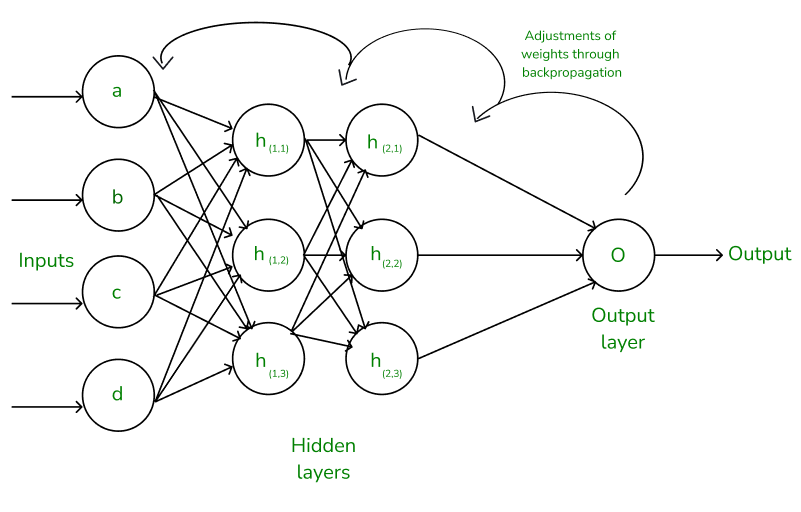
\includegraphics[width=0.5\textwidth]{Images/Frame-13.png}
    \caption{Diagrama ilustrativo del proceso de entrenamiento y retropropagación. \textit{Fuente: Imagen tomada de GeeksforGeeks, recuperada de \url{https://www.geeksforgeeks.org/backpropagation-in-neural-network/}.}}
    \label{fig:Backpropagaion}
\end{figure}

\vspace{7pt}
\subsubsection{iv. Tipos de Aprendizaje}
El \textit{Machine Learning} (ML) comprende un conjunto de técnicas y algoritmos que permiten a las máquinas aprender de los datos y realizar predicciones o tomar decisiones sin estar explícitamente programadas para cada tarea~\cite{elementosIA}. Una de las distinciones fundamentales dentro del ML se basa en el tipo de datos disponibles durante el entrenamiento, específicamente en si esos datos incluyen o no etiquetas o resultados esperados~\cite{sanchez}. De esta forma, se clasifican los enfoques de aprendizaje en cuatro categorías principales: \textbf{supervisado}, \textbf{no supervisado}, \textbf{semisupervisado} y \textbf{por refuerzo}.
\begin{itemize}
    \item \textbf{Aprendizaje Supervisado}: Este tipo de aprendizaje se basa en un conjunto de datos etiquetado, en el que cada instancia contiene características (\textit{features}) y un resultado conocido (\textit{target}) ~\cite{choi2020introduction}. El objetivo es que el modelo aprenda una función de mapeo $f(x) = y$, $x$ representa las entradas y $y$ la salida esperada. Para dar un ejemplo, pensemos en una empresa inmobiliaria que busca predecir el precio de una casa según su número de habitaciones, area en metros cuadrados y ubicación puede utilizar aprendizaje supervisado entrenando un modelo con ejemplos historicos de ventas. El conjunto de datos se divide usualmente en subconjuntos de entrenamiento, validación y prueba, para ajustar, afinar y evualuar el modelo, respectivamente. Las tareas tipicas en este enfoque incluyen:
    \begin{itemize}
    \item\textbf{Regresión}: predicción de valores numéricos continuos (por ejemplo, precios de viviendas).
    \item\textbf{Clasificación}: predicción de categorias discretas (por ejemplo, rango de precios como (0-125k), (125-250k), etc.).    
    \end{itemize}
    \item \textbf{No Supervisado}: A diferencia del aprendizaje supervisado, este enfoque no cuenta con etiquetas o salidas conocidas asociadas a los datos. Es decir, el modelo no tiene una \textquotedblleft respuesta correcta\textquotedblright~que pueda utilizar como guia durante el entrenamiento. En su lugar, debe analizar los datos para identificar patrones subyacentes,estructuras o agrupaciones naturales presentes en ellos. El objetivo es encontrar representaciones útiles de los datos que permiten descubrir relaciones desconocidos o inferir características relevantes sin intervención humana directa ~\cite{choi2020introduction}. \\[2pt]
    Este tipo de aprendizaje es especialmente útil en contextos donde obtener etiquetas es costoso y lento. En muchos casos de la vida real usando este metodo, como grandes bases de datos de clientes, imágenes, secuencias genéticas o registros médicos, se dispone de gran cantidad de informacíón sin clasificar, por lo que los algoritmos no supervisados resultan clave para el análisis exploratiorio y la extración automatica de conocimiento. \\[2pt]
    Las tareas más comunes dentro del aprendizaje no supervisado son:
    \begin{itemize}
        \item \textbf{Clustering (agrupamiento)}: agrupación de datos similares en clústeres basándose en sus características. Por ejemplo un algoritmo podría identificar subconjuntos de viviendas similares sin haber sido informado de categorías específicas.
        \item\textbf{Asociación}: descubrimiento de reglas o correlaciones frecuentes entre características. Útil para entender concurrencias comunes entre variables.
        \item\textbf{Detección de anomalías}: identificacíon de instancias atípicas o fuera de lo común, como precios de vivienda inusualmente altos en un vecindario.
    \end{itemize}
    Este tipo de aprendizaje es valioso cuando etiquetar datos resulta cosotoso o inviable, permitiendo extraer conocimiento directamente de la estructura de los datos.
\end{itemize}
\begin{figure}[H]
\centering
\begin{tikzpicture}[scale=0.8]
    % Supervised Learning (Izquierda)
    \begin{scope}[xshift=-6cm]
        % Ejes
        \draw[thick, ->] (0,0) -- (5,0);
        \draw[thick, ->] (0,0) -- (0,4);
        
        % Puntos rojos (clase 1)
        \foreach \x/\y in {0.5/0.8, 0.8/1.2, 1.2/0.6, 0.6/1.5, 1.0/1.8, 0.4/2.1, 0.9/2.3, 1.3/1.9, 0.7/2.7, 1.1/2.5}
            \fill[red] (\x,\y) circle (2pt);
        
        % Puntos azules (clase 2)
        \foreach \x/\y in {2.5/2.8, 2.8/3.2, 3.2/2.6, 2.6/3.5, 3.0/2.2, 2.4/2.4, 2.9/1.8, 3.3/2.1, 2.7/1.5, 3.1/1.9, 3.5/2.3, 3.8/2.7, 3.4/3.1, 2.2/3.0}
            \fill[blue] (\x,\y) circle (2pt);
        
        % Línea de decisión (discontinua)
        \draw[thick, dashed, black] (1.8,0.2) -- (2.2,3.8);
        
        % Título
        \node[below] at (2.5,-0.3) {\textbf{Supervised learning}};
    \end{scope}
    
    % Línea divisoria vertical
    \draw[thick] (0,-0.5) -- (0,4.5);
    
    % Unsupervised Learning (Derecha)
    \begin{scope}[xshift=1cm]
        % Ejes
        \draw[thick, ->] (0,0) -- (5,0);
        \draw[thick, ->] (0,0) -- (0,4);
        
        % Primer cluster (círculo izquierdo)
        \draw[thick, gray, dashed] (1.2,2.0) circle (0.8);
        \foreach \x/\y in {0.8/1.8, 1.0/2.2, 1.4/1.9, 1.3/2.3, 0.9/2.0, 1.5/2.1, 1.1/1.7, 1.6/1.8}
            \fill[gray] (\x,\y) circle (2pt);
        
        % Segundo cluster (círculo derecha-arriba)
        \draw[thick, gray, dashed] (3.5,3.0) circle (0.7);
        \foreach \x/\y in {3.2/2.8, 3.4/3.2, 3.8/2.9, 3.7/3.3, 3.3/3.0, 3.9/3.1, 3.5/2.7, 3.1/3.1}
            \fill[gray] (\x,\y) circle (2pt);
        
        % Tercer cluster (círculo derecha-abajo)
        \draw[thick, gray, dashed] (3.8,1.2) circle (0.6);
        \foreach \x/\y in {3.5/1.0, 3.7/1.4, 4.1/1.1, 4.0/1.5, 3.6/1.2, 4.2/1.3, 3.8/0.9}
            \fill[gray] (\x,\y) circle (2pt);
        
        % Puntos dispersos
        \foreach \x/\y in {0.5/0.5, 2.0/0.8, 4.3/2.2, 1.8/3.5}
            \fill[gray] (\x,\y) circle (2pt);
        
        % Título
        \node[below] at (2.5,-0.3) {\textbf{Unsupervised learning}};
    \end{scope}
\end{tikzpicture}

\caption{Ejemplo gráfico comparativo de algoritmos de aprendizaje supervisado y no supervisado.\textit{Fuente: Elaboración propia.}}
\label{fig:aprendizaje-supervisado-no-supervisado}
\vspace{2mm}

\small\textit{Nota:} En la parte izquierda (aprendizaje supervisado), la línea discontinua representa una frontera de decisión aprendida a partir de datos etiquetados. En cambio, el gráfico derecho (aprendizaje no supervisado) muestra cómo los algoritmos agrupan automáticamente los datos sin etiquetas previas, basándose únicamente en similitud o cercanía.

\end{figure}
\subsection{b. Nociones de Redes Neuronales (NN)}
\vspace{5pt}

\subsubsection{i.Componentes de la Red: Neuronas, Capas, Pesos,Activación} 
\vspace{3pt}
Las \textit{Redes Neuronales (NN)} son una clase de modelos matemáticos y computacionales diseñados para reconocer patrones y relaciones complejas entre datos~\cite{sanchez}. Se inspiran libremente en el funcionamiento del cerebro humano, particularmente en la forma en que las neuronas biológicas se comunican a través de sinapsis para procesar información.

En términos generales, una red neuronal está compuesta por un conjunto de unidades computacionales llamadas \textbf{neuronas artificiales}, organizadas en capas conectadas entre sí mediante enlaces ponderados~\cite{elementosIA}. En nuestro contexto actual acerca del aprendizaje automático, las redes neuronales forman la base del \textbf{aprendizaje profundo} (\textit{Deep Learning}), especialmente cuando estas redes poseen múltiples capas.

\begin{itemize}
    \item\textbf{Neuronas}: son las unidades básicas de procesamiento de la red. Cada neurona recibe entradas numéricas, las combina mediante una operación de suma ponderada y aplica una función de activación para determinar su salida. Esta salida se propaga hacia las neuronas de la siguiente capa. Aunque una sola neurona tiene capacidad limitada, al ser organizadas en grandes conjuntos y capas interconectadas, adquieren una potencia por sí solas ~\cite{datacamp_redes}.

    \item\textbf{Capas}:
    \begin{itemize}
        \item \textbf{Capa de entrada}: Corresponde a los datos que se introducen en la red. Cada nodo representa una característica del conjunto de datos( por ejemplo: color, tamaño,edad,etc.):
        \item\textbf{Capas ocultas}: Las capas ocultas de una red neuronal contienen unidades no observables y son las encargadas de transformar la información mediante operaciones sucesivas. En redes profundas (\textit{deep networks}), estas capas pueden ser numerosas, lo que permite modelar funciones altamente complejas.
        \item\textbf{Capa de salida}: Genera la predicción final del modelo, ya sea una clase, un valor numérico o una distribución de probabilidad, dependiendo del problema a resolver.
    \end{itemize}

   \item\textbf{Pesos y Sesgos (Biases)}:
    \begin{itemize}
        \item \textbf{Pesos}: Cada conexión entre neuronas tiene un peso asociado, que representa la fuerza o importancia de esa conexión. Durante el proceso de entrenamiento, estos pesos son ajustados iterativamente para que la red aprenda de los datos y reduzca su error en las predicciones.
        \item \textbf{Sesgos}: Son valores adicionales que se suman a la entrada de la función de activación de cada neurona. Actúan como un parámetro de ajuste adicional, permitiendo desplazar la salida de una neurona y mejorar la capacidad de aprendizaje del modelo.
    \end{itemize}
    \item \textbf{Funciones de Activación}: Estas funciones determinan la salida de cada neurona a partir de su entrada ponderada. Son importantes porque introducen no linealidades en el modelo, lo que nos permite que las redes neuronales aprendan relaciones complejas más allá de simples combinaciones lineales ~\cite{datacamp_redes}. Algunas de las funciones de activación más comunes incluyen:
    \begin{itemize}
        \item \textbf{ReLU (Rectified Linear Unit)}: Devuelve cero si la entrada es negativa, y la entrada misma si es positiva. Es eficiente y muy utilizada en redes profundas.
        \item \textbf{Sigmoide}: Convierte las entradas en valores entre 0 y 1, útil en tareas de clasificación binaria. 
        \item \textbf{Tanh (Tangente Hiperbólica)}: Similar a la sigmoide pero con salida entre -1 y 1, centrada en cero, lo cual puede favorecer una convergencia más rápida durante el entrenamiento.
    \end{itemize}
\end{itemize}
\begin{figure}[H]
    \centering
    \begin{tikzpicture}[scale=1.5]
        % Nodos de entrada
        \draw (0,2) circle (0.2) node {$x_1$};
        \draw (0,1) circle (0.2) node {$x_2$};
        \draw (0,0) circle (0.2) node {$x_3$};
        
        % Nodos ocultos
        \draw (2,2) circle (0.2) node {$h_1$};
        \draw (2,1) circle (0.2) node {$h_2$};
        \draw (2,0) circle (0.2) node {$h_3$};
        
        % Nodo de salida
        \draw (4,1) circle (0.2) node {$y$};
        
        % Conexiones
        \draw (0.2,2) -- (1.8,2);
        \draw (0.2,2) -- (1.8,1);
        \draw (0.2,2) -- (1.8,0);
        \draw (0.2,1) -- (1.8,2);
        \draw (0.2,1) -- (1.8,1);
        \draw (0.2,1) -- (1.8,0);
        \draw (0.2,0) -- (1.8,2);
        \draw (0.2,0) -- (1.8,1);
        \draw (0.2,0) -- (1.8,0);
        
        \draw (2.2,2) -- (3.8,1);
        \draw (2.2,1) -- (3.8,1);
        \draw (2.2,0) -- (3.8,1);
        
        % Etiquetas
        \node at (0,2.5) {Entrada};
        \node at (2,2.5) {Oculta};
        \node at (4,1.5) {Salida};
    \end{tikzpicture}
\caption{Estructura típica de una red neuronal, que incluye la capa de entrada, varias capas ocultas y la capa de salida. \textit{Fuente: Elaboración propia.}}
    \label{fig:red-neuronal-tikz}
\end{figure}
\subsubsection{ii. Inferencia por propagación hacia adelante}
La propagación hacia adelante (\textit{forward propagation}) es el proceso por el que una red neuronal transforma los datos de entrada en predicciones o salidas~\cite{datacamp_redes}. En términos técnicos, es el cálculo secuencial que mueve los datos desde la capa de entrada, a través de las capas ocultas y, finalmente, a la capa de salida~\cite{nvidia}. Durante este recorrido, los datos se transforman mediante conexiones ponderadas y funciones de activación, lo que permite a la red captar patrones complejos. \\
La importancia de la propagación hacia adelante radica en que es el mecanismo principal por el cual el modelo genera sus predicciones basadas en los parámetros que ha aprendido durante el entrenamiento que se le da. Sin este proceso, no sería posible evaluar cómo se comporta la red ante nuevos datos sin medir su desempeño. Además, la propagación hacia adelante es esencial para calcular la función de pérdida, que es la medición de los errores entre las predicciones y los valores reales. Esta información es usada posteriormente durante la retropropagación  para ajustar los pesos de la red y mejorar su precisión.
\begin{figure}[H]
    \centering
    \scalebox{0.8}{
    \begin{tikzpicture}[
        neuron/.style={circle, draw=black, fill=blue!20, minimum size=12mm},
        arrow/.style={-{Stealth[length=3mm, width=2mm]}, thick, blue},
        layerlabel/.style={font=\bfseries, align=center}
    ]

    % Capas
    % Capa Entrada
    \node[layerlabel] (inputlabel) at (0,4) {Entrada};
    \node[neuron] (I1) at (0,3) {$x_1$};
    \node[neuron] (I2) at (0,2) {$x_2$};
    \node[neuron] (I3) at (0,1) {$x_3$};

    % Capa Oculta
    \node[layerlabel] (hiddenlabel) at (5,5) {Oculta};
    \node[neuron] (H1) at (5,3.5) {$h_1$};
    \node[neuron] (H2) at (5,2.5) {$h_2$};
    \node[neuron] (H3) at (5,1.5) {$h_3$};

    % Capa Salida
    \node[layerlabel] (outputlabel) at (10,3) {Salida};
    \node[neuron] (O1) at (10,2) {$y$};

    % Conexiones Entrada -> Oculta
    \draw[arrow] (I1) -- (H1);
    \draw[arrow] (I1) -- (H2);
    \draw[arrow] (I1) -- (H3);

    \draw[arrow] (I2) -- (H1);
    \draw[arrow] (I2) -- (H2);
    \draw[arrow] (I2) -- (H3);

    \draw[arrow] (I3) -- (H1);
    \draw[arrow] (I3) -- (H2);
    \draw[arrow] (I3) -- (H3);

    % Conexiones Oculta -> Salida
    \draw[arrow] (H1) -- (O1);
    \draw[arrow] (H2) -- (O1);
    \draw[arrow] (H3) -- (O1);


    \end{tikzpicture}
    }
    \caption{Propagación hacia adelante (Forward propagation) en una red neuronal simple.\textit{Fuente: Elaboración propia}}
    \label{fig:forward_propagation}
\end{figure}

\subsubsection{iii. Entrenamiento}
\vspace{3pt}
El entrenamiento de una red neuronal es un proceso donde ajustamos los pesos internos de la red con el fin de minimizar la diferencia entre las predicciones de la red y los valores reales esperados. Este proceso permite que la red aprenda a representar patrones presentes en los datos, generalizando su conocimiento para realizar predicciones sobre datos no vistos~\cite{zhou2020graph}. El entrenamiento está compuesto por dos fases principales: la evaluación del error, por medio de una \textbf{función de pérdida}, y la \textbf{actualización de los pesos} usando el algoritmo de \textit{propagación hacia atrás} (\textit{backpropagation})~\cite{nvidia}.
\begin{itemize}
\item\textbf{1. Función de pérdida}:\newline
Es una función de pérdida cuantificada para saber qué tan bien o mal está funcionando una red. Calcula la diferencia entre la salida predicha por la red y el valor real esperado ~\cite{zhou2020graph}. El objetivo del entrenamiento es minimizar esta función de perdida mediante la actualización iterativa de los pesos. \newline Algunas funciones comunes son:
\begin{itemize}
    \item \textbf{Error cuadrático medio (MSE)}: Utilizada en tareas de regresión, se define como : $\mathcal{L}_{MSE} = \frac{1}{n} \sum_{i=1}^{n}(y_i - \hat{y}_i)^2$
    \item \textbf{Entropía cruzada}: Utilizada para clasificación, especialmente con salidas probabilísticas. Si se tiene una salida verdadera $y$ y una predicción $\hat{y}$, la pérdida es: $\mathcal{L}_{CE} = -\sum y \log(\hat{y})$
\end{itemize}

\item\textbf{2. Propagación hacia atrás (Backpropagation)}:\newline
Este es un algoritmo central para entrenar redes neuronales. Utiliza el cálculo de derivadas (gradientes) para actualizar los pesos de la red en dirección contraria a la propagación hacia adelante ~\cite{nvidia}. El proceso sigue los siguientes pasos:
\begin{enumerate}
    \item Se realiza una propagación hacia adelante para obtener las predicciones.
    \item Se calcula la pérdida comparando con los valores reales.
    \item Se aplica la regla de la cadena para propagar el error desde la capa de salida hacia atrás, capa por capa, computando los gradientes parciales con respecto a cada peso.
    \item Se actualizan los pesos mediante un algoritmo de optimización, típicamente descenso del gradiente:$w \leftarrow w - \eta \cdot \frac{\partial \mathcal{L}}{\partial w}$, donde $\eta$ es la tasa de aprendizaje.
\end{enumerate}
Este proceso se repite en multiples iteraciones (\textit{epochs}) sobre el conjunto de entrenamiento. Al finalizar, la red ha ajustado sus parámetros internos para producir predicciones más precisas.

\item \textbf{Regularización y generalización}: \newline
Para evitar el sobreajuste (overfitting), es común introducir técnicas de regularización como \textit{Dropout}, \textit{L2 regulization}, o el uso de validación cruzada. Estas técnicas mejoran la capacidad de generalización del modelo.
\end{itemize}
\begin{figure}[H]
    \centering
    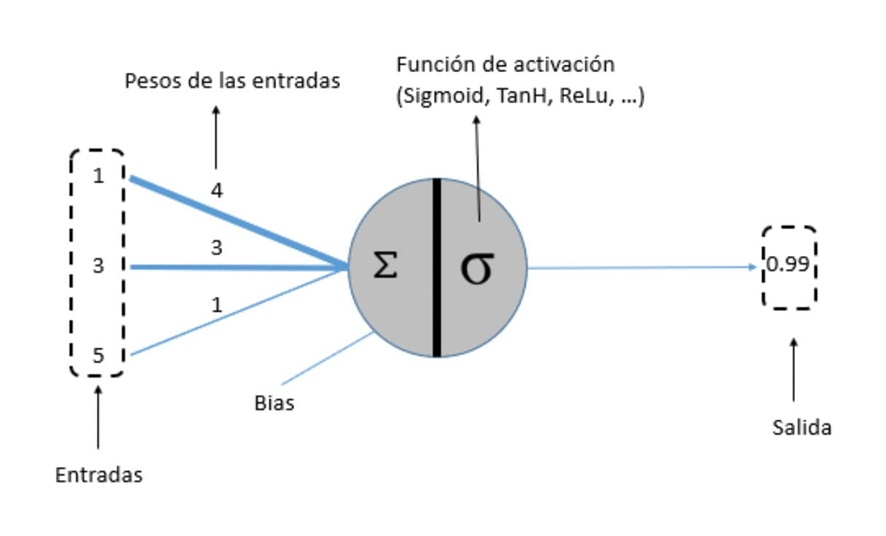
\includegraphics[width=0.5\textwidth]{Images/111-1.jpg}
    \caption{Modelo de una neurona artificial. Cada entrada es multiplicada por un peso, se suma un sesgo (bias) y se aplica una función de activación (como Sigmoid, Tanh o ReLU) para obtener la salida. \textit{Fuente: Imagen tomada de Ángel Villazón, recuperada de \url{https://www.angelvillazon.com/inteligencia-artificial-robotica/entrenamiento-de-redes-neuronales/}.}}
    \label{fig:neurona-artificial}
\end{figure}

\subsection{c. Aplicaciones} 
\vspace{3pt}
Las redes neuronales tienen un amplio uso de aplicaciones practicas que abarcan desde el análisis de imágenes hasta el procesamiento de lenguaje natural ~\cite{hui2021gnn}. Estás aplicaciones aprovechan la capacidad de las redes para aprender representaciones complejas y generalizar a partir de datos de entrenamiento en diferentes contextos del mundo real.
\begin{itemize}
\item \textbf{i. Reconocimiento de Imágenes}; \newline
Las redes neuronales de grafos (GNN) han ampliado las posibilidades en el reconocimiento de imágenes, especialmente cuando estas se representan como grafos, como en el caso de imágenes con superpíxeles o estructuras espaciales irregulares. Permiten tareas como clasificación de objetos, detección de patrones, segmentación y reconocimiento de escritura manuscrita a partir de representaciones gráficas ~\cite{hui2021gnn}. Estas redes son capaces de extraer automáticamente características relevantes mediante el intercambio de información entre nodos conectados, lo cual reduce la necesidad de ingeniería manual de características. Se aplican en visión por computadora basada en grafos, diagnóstico médico (analizando relaciones espaciales en imágenes), vehículos autónomos (procesamiento estructural de escenas), y sistemas inteligentes de vigilancia.


    \item \textbf{ii. Procesamiento de Lenguaje Natural (NLP)}: \newline
    En el campo del procesamiento del lenguaje natural, las redes neuronales han hecho posibles avances significativos gracias a arquitecturas como RNN, LSTM y los modelos de transformadores ~\cite{aws2025nlp}. Estas arquitecturas permiten capturar la estructura y semántica del lenguaje humano, facilitando tareas como traducción automática, análisis de sentimientos, generación de texto, respuesta a preguntas, detección de spam, y clasificación de documentos. Modelos de lenguaje como BERT, GPT y sus derivados se entrenan con enormes cantidades de datos textuales, lo que les permite comprender y generar lenguaje de forma coherente, ofreciendo la base para asistentes virtuales, motores de búsqueda inteligentes y herramientas de apoyo al usuario en tiempo real.

\end{itemize}
\newpage
{\section{Fundamentos y justificación de GNNs}} 
\vspace{5pt}
Las \textbf{Redes neuronales de Grafos} (GNNs, por sus siglas en inglés) son una clase de modelos diseñados específicamente para trabajar con datos estructurados como grafos. Estos modelos extienden la capacidad de las redes neuronales tradicionales al considerar explícitamente la estructura de conexiones entre elementos, permitiendo aprender representaciones útiles de nodos, aristas y del grafo completo. Se han vuelto fundamentales en tareas que involucran relaciones complejas, como redes sociales, conocimiento biomecular, sistemas de recomendación, y más. \\[3pt]
\textbf{a. Definiciones Básicas} \\[3pt]
Un \textbf{grafo} $G = (V, E)$ está compuesto por un conjunto de nodos (vértices) $V$ y un conjunto de aristas (enlaces) $E \subseteq V \times V$. En muchos contextos, tanto los nodos como las aristas están asociados a vectores de características. Por ejemplo, en un grafo de usuarios, cada nodo puede representar a un usuario con atributos como edad, ubicación e intereses, y cada arista puede representar una amistad o interacción.
\begin{figure}[h]
\centering
\begin{tikzpicture}[scale=1.2]

% Nodos simples
\node[circle, draw, fill=blue!20, minimum size=12mm] (A) at (0, 2) {Ana};
\node[circle, draw, fill=green!20, minimum size=12mm] (B) at (3, 3) {Carlos};
\node[circle, draw, fill=yellow!20, minimum size=12mm] (C) at (3, 1) {Luis};
\node[circle, draw, fill=pink!20, minimum size=12mm] (D) at (6, 2) {María};

% Aristas simples
\draw[thick] (A) -- (B) node[midway, above] {Amigos};
\draw[thick] (A) -- (C) node[midway, left] {Trabajo};
\draw[thick] (B) -- (D) node[midway, above] {Pareja};
\draw[thick] (C) -- (D) node[midway, below] {Vecinos};

% Etiquetas
\node at (3, 0) {$G = (V, E)$};
\node at (3, -0.5) {$V = \{Ana, Carlos, Luis, Maria\}$};

\end{tikzpicture}
\caption{Ejemplo grafo simple de usuarios.\textit{Fuente: Elaboración propia.}}
\label{fig:grafo_simple}
\end{figure}

\newpage 
\section{Caso de Estudio GCN} \vspace{10pt}

\subsection{a. Definición y Justificación}

Una Red Convolucional sobre Grafos (GCN, por sus siglas en inglés) es un tipo de red neuronal diseñada para trabajar directamente con estructuras en forma de grafo. A diferencia de las redes tradicionales, que esperan como entrada datos organizados en forma de vectores o matrices (como las imágenes o secuencias), las GCN pueden procesar datos cuya forma natural es un conjunto de nodos conectados por relaciones, como ocurre en redes sociales, mapas de relaciones científicas o redes biológicas.

Las GCN fueron propuestas por Thomas Kipf y Max Welling en 2016~\cite{kipf2016semi}, como una solución para tareas como la clasificación de nodos dentro de un grafo, especialmente en situaciones donde no todos los nodos tienen etiquetas conocidas. Lo innovador de este modelo es que puede aprender a predecir etiquetas utilizando tanto las características de cada nodo como la estructura de conexiones entre ellos, sin necesidad de transformar el grafo en una estructura lineal.

Esto es especialmente útil en problemas donde solo se conoce la clase o etiqueta de algunos pocos nodos, ya que la GCN puede aprovechar las conexiones del grafo para extender esa información a los demás nodos. Además, las GCN permiten realizar este proceso de forma eficiente, utilizando operaciones simples pero efectivas que se pueden aplicar directamente sobre la estructura del grafo.

\subsection{b. Características Distintivas}

Las GCN tienen varias propiedades clave que las hacen diferentes a otros modelos de aprendizaje automático. A continuación se explican junto con un ejemplo ilustrativo basado en una red de recomendación de películas:

\begin{itemize}
    \item \textbf{Agregación de información local:} en cada capa, un nodo combina su información con la de sus vecinos directos. Por ejemplo, si una persona no ha indicado sus gustos de películas, pero sus amigos sí lo han hecho, se puede usar esa información para inferir qué películas le podrían gustar.

    \item \textbf{Uso de los mismos parámetros:} la misma matriz de pesos se aplica a todos los nodos. Esto permite detectar patrones similares en distintas partes del grafo. En nuestro ejemplo, sin importar si un nodo representa a “Ana” o “Luis”, el modelo usa los mismos parámetros para actualizar su representación.

    \item \textbf{Independencia del orden de los vecinos:} como el orden de los amigos no afecta a quién me influye más o menos, las operaciones como el promedio son ideales para que el modelo funcione sin importar cómo estén ordenados los vecinos.

    \item \textbf{Generalización a distintos grafos:} una GCN puede usarse en grafos con estructuras diferentes. Por ejemplo, si se entrena en una red de usuarios de una ciudad, puede aplicarse luego a otra red de usuarios de otra ciudad que tengan conexiones y gustos similares.
\end{itemize}

\begin{figure}[H]
    \centering
    \begin{tikzpicture}[every node/.style={circle, draw, minimum size=1cm}, node distance=2cm]
        \node[fill=yellow!30] (A) at (0,0) {¿?};
        \node[fill=blue!20] (B) at (-2,1.5) {Si};
        \node[fill=blue!20] (C) at (2,1.5) {Si};
        \node[fill=blue!20] (D) at (-2,-1.5) {Si};
        \node[fill=red!20] (E) at (2,-1.5) {No};

        \draw (A) -- (B);
        \draw (A) -- (C);
        \draw (A) -- (D);
        \draw (A) -- (E);
    \end{tikzpicture}
    \caption{Ejemplo de GCN en una red de recomendación. El nodo central no tiene información directa, pero puede inferirse por los gustos de sus amigos (Si = le gusta el cine, No = no le gusta) \textit{Fuente: Elaboración propia}.}
    \label{fig:movie_recommendation}
\end{figure}

\vspace{0.5em}
En la Figura, el nodo central representa a una persona la cual se desconoce su gusto por el cine (¿?). Sin embargo, tres de sus amigos ya indicaron que les gusta el cine, y uno que no. Gracias a la GCN, el nodo puede actualizar su representación combinando estas señales y así predecir si probablemente también le gusten las películas.




\subsection{c. Modelo de Propagación}

El modelo de propagación define cómo se actualizan las representaciones de los nodos usando tanto sus características como las conexiones en el grafo. Esto se hace combinando dos elementos: la matriz de adyacencia (que indica quién está conectado con quién) y la matriz de características (que guarda los datos de cada nodo).

\subsubsection{i. Features}

Cada nodo $i$ tiene un vector de características $\mathbf{x}_i \in \mathbb{R}^F$, donde $F$ es el número de atributos que describen ese nodo. Por ejemplo, en un grafo de artículos científicos como Cora, estos atributos pueden indicar qué palabras aparecen en cada artículo.

Si hay $N$ nodos, se puede representar toda la información en una sola matriz $X \in \mathbb{R}^{N \times F}$, donde cada fila corresponde a un nodo y cada columna a una característica.

\subsubsection{ii. Matriz de Adyacencia}

La \textit{matriz de adyacencia}, denotada como $A \in \mathbb{R}^{N \times N}$. Esta matriz tiene un valor $A_{ij} = 1$ si existe una conexión directa (una arista) entre el nodo $i$ y el nodo $j$, y un valor $A_{ij} = 0$ si no hay conexión.

Sin embargo, en el modelo GCN también se quiere que cada nodo tenga en cuenta su propia información al actualizarse. Para lograr esto, se agregan conexiones del nodo consigo mismo, llamadas \textit{autoconexiones} o \textit{self-loops}. Esto se hace sumando la matriz identidad $I_N$ a la matriz de adyacencia original:

\[
\hat{A} = A + I_N
\]

Esta nueva matriz $\hat{A}$ se utiliza en los cálculos posteriores para la propagación de información.


\subsubsection{iii. Matriz de Pesos}

La \textit{matriz de pesos}, denotada como $W^{(l)}$, se utiliza para transformar las representaciones de los nodos en cada capa $l$ de la GCN. Esta transformación es lineal y permite que el modelo aprenda a combinar y proyectar las características de los nodos a un nuevo espacio de representación.

Cada capa tiene su propia matriz de pesos, que se ajusta automáticamente durante el entrenamiento. Esta matriz actúa sobre la información agregada de los vecinos y del propio nodo, permitiendo capturar patrones útiles para la tarea de aprendizaje.

La fórmula general para calcular la salida de una capa es:

\[
H^{(l+1)} = \sigma\left( \hat{D}^{-1/2} \hat{A} \hat{D}^{-1/2} H^{(l)} W^{(l)} \right)
\]

donde:
\begin{itemize}
    \item $H^{(0)} = X$, la matriz de características iniciales de los nodos,
    \item $\hat{A}$ es la matriz de adyacencia con autoconexiones,
    \item $\hat{D}$ es la matriz diagonal de grados asociada a $\hat{A}$,
    \item $\sigma$ es una función de activación no lineal.
\end{itemize}

\subsubsection{iv. Normalización y Activación}

El término $\hat{D}^{-1/2} \hat{A} \hat{D}^{-1/2}$ realiza una \textit{normalización simétrica} sobre la matriz de adyacencia modificada $\hat{A}$. Esta normalización ajusta los valores de las conexiones en función del grado de los nodos, es decir, del número total de conexiones que tiene cada nodo, incluyendo las autoconexiones.

Para construir la matriz $\hat{D}$, se calcula la suma de cada fila de $\hat{A}$ y se coloca ese valor en la diagonal correspondiente. De esta forma, $\hat{D}_{ii} = \sum_j \hat{A}_{ij}$. El objetivo de esta normalización es evitar que los nodos con muchos vecinos dominen el proceso de agregación, manteniendo un equilibrio entre la influencia de todos los nodos.

La función $\sigma$ representa una activación no lineal que se aplica después de la agregación y la transformación lineal. En las capas ocultas se suele usar la función ReLU, que introduce no linealidad al modelo. En la capa final, si el problema es de clasificación, se utiliza la función softmax para obtener una distribución de probabilidades sobre las posibles clases.

\subsection{d. Agregación de Features y Transformación de Nodos}

En cada capa de una GCN, los nodos actualizan sus representaciones combinando sus propias características con las de sus vecinos. Este proceso se conoce como \textit{agregación de features}. A medida que el modelo avanza por las capas, cada nodo puede acceder a información de vecinos más lejanos dentro del grafo.

La representación del nodo $v$ en la capa $l+1$ se calcula como:

\[
\mathbf{h}_v^{(l+1)} = \sigma \left( \sum_{u \in \mathcal{N}(v) \cup \{v\}} \frac{1}{\sqrt{d_v d_u}} \mathbf{h}_u^{(l)} W^{(l)} \right)
\]

donde $\mathcal{N}(v)$ es el conjunto de vecinos del nodo $v$, y $d_v$ es su grado (incluyendo la autoconexión). En esta fórmula, cada nodo combina las representaciones de sus vecinos y las suyas propias, las transforma linealmente con $W^{(l)}$, y aplica una función de activación.

Este proceso se repite en múltiples capas. Con cada nueva capa, el nodo incorpora información de una vecindad más amplia, lo que permite construir una representación final que refleja tanto sus atributos individuales como la estructura del grafo a su alrededor.


\subsection{e. Aplicaciones}

\subsubsection{i. Redes Sociales}

Las redes sociales digitales, como Facebook, Twitter o Instagram, pueden modelarse naturalmente como grafos, donde cada nodo representa a un usuario y cada arista representa una relación social, como amistad, seguimiento o interacción frecuente. Esta estructura gráfica permite aplicar modelos GCN para realizar diversas tareas que requieren entender tanto las características de los usuarios como su posición dentro de la red.

Una aplicación común es la \textit{clasificación de usuarios}, donde se desea predecir intereses, grupos a los que pertenece una persona o su probabilidad de interactuar con ciertos contenidos. Las GCN permiten usar no solo los datos propios de cada usuario (como sus publicaciones, gustos o edad), sino también los datos de sus amigos o contactos cercanos. Esto es especialmente útil cuando un usuario tiene poca información disponible: su vecindad en el grafo puede ser suficiente para hacer una predicción.

Otras aplicaciones incluyen:

\begin{itemize}
    \item \textbf{Detección de comunidades:} identificar grupos densamente conectados que comparten características similares.
    \item \textbf{Predicción de vínculos:} anticipar la aparición de nuevas relaciones entre usuarios, como sugerencias de amistad.
    \item \textbf{Filtrado de contenido:} estimar la relevancia de publicaciones basándose en la estructura social y las interacciones previas.
\end{itemize}

\begin{figure}[H]
    \centering
    \begin{tikzpicture}[every node/.style={circle, draw, minimum size=1cm}, scale=1.1]

        % Nodos
        \node[fill=yellow!30] (A) at (0,0) {Tú};
        \node[fill=blue!20] (B) at (-2,1.5) {Fútbol};
        \node[fill=blue!20] (C) at (2,1.5) {Fútbol};
        \node[fill=blue!20] (D) at (-2,-1.5) {Fútbol};
        \node[fill=red!20] (E) at (2,-1.5) {No};

        % Aristas
        \draw (A) -- (B);
        \draw (A) -- (C);
        \draw (A) -- (D);
        \draw (A) -- (E);

    \end{tikzpicture}
    \caption*{
    \textit{Fuente: Creacion propia}
    }
\end{figure}

\vspace{0.5em}
El nodo central representa a un usuario sin etiqueta conocida. Al estar conectado con tres amigos interesados en fútbol, una GCN puede predecir que probablemente él también comparta ese interés.

\newpage 
{\section{Ejemplo Demostrativo de GCN }} \vspace{10pt}

\subsection{a. Descripción del Problema (el esperado es una clasificación de nodos)} 



\subsection{b. Obtención del Dataset}



\subsection{c. Configuración de la GCN} 



\subsection*{d. Descripción del algoritmo e implementación en Python}



\subsection*{e. Visualización y Análisis de Resultados}

\newpage
\section{Conclusión}

\newpage
\section{Referencias}
\nocite{*}
\printbibliography
\newpage 
\section{Anexos}
\vspace{10pt}
\subsection{Anexo A: Glosario de Términos y Conceptos Adicionales}
\subsubsection{Ejemplo de Cálculo de Propagación hacia Adelante}
Dado un vector de entrada \(x = [0.5, -0.3]\), pesos \(W\) y sesgo \(b\):

\[
W = \begin{bmatrix}
0.2 & -0.4 \\
0.7 & 0.1 
\end{bmatrix}, \quad
b = \begin{bmatrix}
0.1 \\
-0.2
\end{bmatrix}
\]

La salida \(y\) se calcula como:
\[
y = \text{ReLU}(Wx + b)
\]

\[
Wx = \begin{bmatrix}
0.2 & -0.4 \\
0.7 & 0.1 
\end{bmatrix}
\begin{bmatrix}
0.5 \\
-0.3
\end{bmatrix}
= \begin{bmatrix}
(0.2)(0.5) + (-0.4)(-0.3) \\
(0.7)(0.5) + (0.1)(-0.3)
\end{bmatrix}
= \begin{bmatrix}
0.1 + 0.12 \\
0.35 - 0.03
\end{bmatrix}
= \begin{bmatrix}
0.22 \\
0.32
\end{bmatrix}
\]

\[
y = \text{ReLU}\left(
\begin{bmatrix}
0.22 \\
0.32
\end{bmatrix} + 
\begin{bmatrix}
0.1 \\
-0.2
\end{bmatrix}
\right)
= \text{ReLU}
\begin{bmatrix}
0.32 \\
0.12
\end{bmatrix}
= \begin{bmatrix}
0.32 \\
0.12
\end{bmatrix}
\]

---

\subsubsection{Glosario de Términos}
\begin{description}
    \item[\textbf{Algoritmo de Optimización}] Método matemático utilizado para minimizar o maximizar una función objetivo, comúnmente la función de pérdida en machine learning.
    
    \item[\textbf{Batch}] Subconjunto de datos de entrenamiento que se procesa simultáneamente durante una iteración del algoritmo de entrenamiento.
    
    \item[\textbf{Cross-validation (Validación Cruzada)}] Técnica estadística para evaluar la capacidad de generalización de un modelo dividiendo los datos en múltiples particiones.
    
    \item[\textbf{Dropout}] Técnica de regularización que consiste en desactivar aleatoriamente algunas neuronas durante el entrenamiento para prevenir el sobreajuste.
    
    \item[\textbf{Epoch}] Una pasada completa a través de todo el conjunto de datos de entrenamiento.
    
    \item[\textbf{Feature Engineering}] Proceso de selección, modificación o creación de variables (features) a partir de datos en bruto para mejorar el rendimiento del modelo.
    
    \item[\textbf{Gradient Descent}] Algoritmo de optimización iterativo usado para encontrar el mínimo de una función calculando sus gradientes.
    
    \item[\textbf{Hiperparámetros}] Parámetros de configuración del modelo que se establecen antes del entrenamiento y no se aprenden automáticamente.
    
    \item[\textbf{Learning Rate (Tasa de Aprendizaje)}] Hiperparámetro que controla qué tan grande es el paso que da el algoritmo en cada iteración hacia el mínimo de la función de pérdida.
    
    \item[\textbf{Overfitting (Sobreajuste)}] Fenómeno donde el modelo aprende demasiado bien los datos de entrenamiento pero falla al generalizar a datos nuevos.
    
    \item[\textbf{Underfitting (Subajuste)}] Situación donde el modelo es demasiado simple para capturar la estructura subyacente de los datos.
\end{description}
\subsection{Funciones de Activación Adicionales}

Además de las funciones mencionadas en el documento principal, existen otras funciones de activación relevantes:

\begin{itemize}
    \item \textbf{Leaky ReLU}: Variante de ReLU que permite un pequeño gradiente cuando la entrada es negativa: $f(x) = \max(0.01x, x)$
    
    \item \textbf{ELU (Exponential Linear Unit)}: $f(x) = \begin{cases} x & \text{si } x > 0 \\ \alpha(e^x - 1) & \text{si } x \leq 0 \end{cases}$
    
    \item \textbf{Swish}: Función autodescubierta por Google: $f(x) = x \cdot \sigma(x)$, donde $\sigma$ es la función sigmoide.
    
    \item \textbf{Softmax}: Utilizada en la capa de salida para problemas de clasificación multiclase: $f(x_i) = \frac{e^{x_i}}{\sum_{j=1}^{K} e^{x_j}}$
\end{itemize}
\end{document}

